\def\CC{{C\nolinebreak[4]\hspace{-.05em}\raisebox{.4ex}{\tiny\bf ++}}}

\begin{frame}\frametitle{}
\vspace*{0.2in}
\centerline{\textrm{{\huge\bfseries\color{myOrange} \textit{MIRGE-Com}}}}
\smallskip
\centerline{\textrm{{\huge\bfseries\color{myOrange} Performance Snapshot}}}
\smallskip
\smallskip
\centerline{\textrm{{\large\bfseries{Fri@CEESD - February 26, 2021}}}}
%\centerline{\textrm{{\big\bfseries\color{myOrange} Anatomy of a large scale prediction}}}
\vspace*{0.2in}
%\hrule
%\begin{center}
%\includegraphics[width=0.85\textwidth]{Figures/TitleFig.pdf}
%\end{center}
%\hrule
\begin{center}
\vspace*{0.4in}
\cPI{Mike Campbell}
\end{center}
\end{frame}

\begin{frame}\frametitle{Outline}
\begin{itemize}
\item Performance - why do users care?
\item Y1 Simulation targets
\item Performance snapshots of \textit{MIRGE-Com}
\item Projected resource needs for Y1
\item Summary
\end{itemize}
\end{frame}

% Why does the user care about performance?
% Get the *simulation work* done in time to matter
% Get it done within cost (resource = $$)

% Given a fixed resource, what's the "biggest" simulation that can be done?
% How much faster can the simulation work get done with increased resources?

% Computational resource?
% number of PU * wallclock time

% Simulation work?
% Discrete domain size * simulated time
\begin{frame}\frametitle{Performance - why do users care?}
\begin{multicols}{2}
%\begin{itemize}
%\item Typical users:
\begin{itemize}
\item Usual: Need \textit{simulation work} done in time to matter
\item Less usual: Need simulation work done within budget (\$)
%\end{itemize}
\columnbreak
\item Scaling \textit{computational resource}:
\begin{itemize}
\item How fast can the simulation work be done? (strong scaling, fixed total work)
\item How much simulation work can be done? (weak scaling, fixed work / PU)
\end{itemize}
\end{itemize}
\end{multicols}
\begin{center}
\vspace{10pt}
Computational resource: Number of Processing Unit $\times$ Wallclock Time $(N_p \times T_w)$\\
\vspace{10pt}
Simulation work: Simulation Size $\times$ Total Simulated Time $(C_e \times N_e \times N_s \times \Delta{T_s})$
\end{center}
\end{frame}

% What simulation work?
% Domain description
% simulated time = Flowthrough timescale ()
% Current estimates on discretized domain size
% Show Mike's spreadsheet on dt vs. h/p^2
% Show Wyatt's increasing resolution grids
% Reason to believe that we'll have ~1M elements, 1e-9 DT
% Features?  Inviscid, inviscid + shock capt, NS?
\begin{frame}\frametitle{What simulation work?}
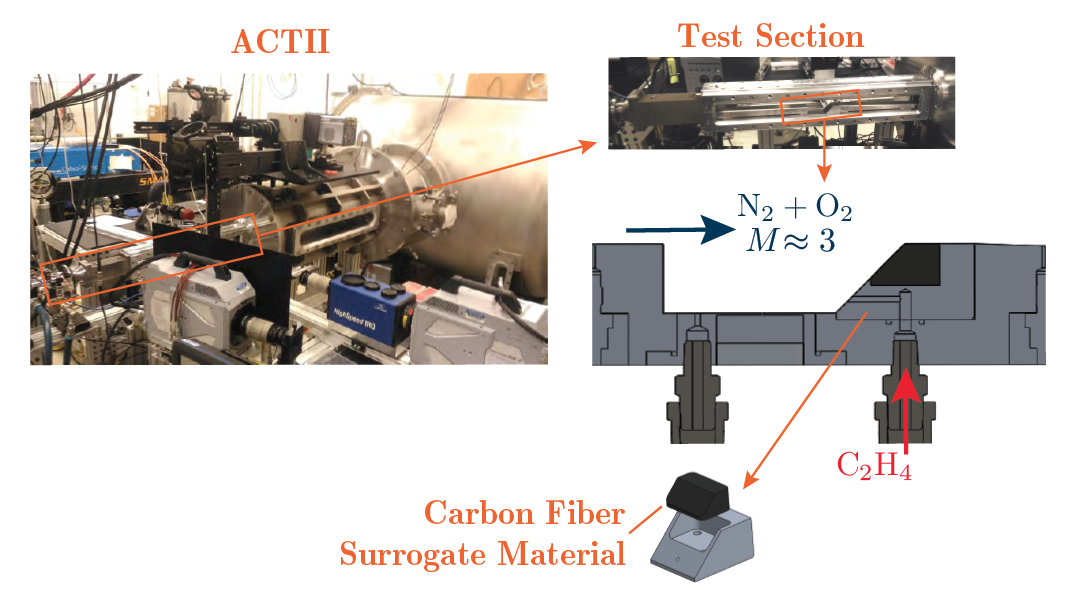
\includegraphics[width=\textwidth]{figures/actii.png}
\begin{center}
 \prj{\tiny}{Freund}
\end{center}
\end{frame}

\begin{frame}\frametitle{What simulation work?}
\begin{multicols}{2}
\begin{itemize}
\item Inviscid flow (Euler)
\item Mach 1-3 (shock capturing)
\item Fuel/Air (Pyro mixtures)
\item Combustion (Pyro chemistry)
\item Navier-Stokes (WIP)
\item Wall model \& interaction (WIP)
\end{itemize}
\columnbreak
% todo: truncated nozzle grid pic
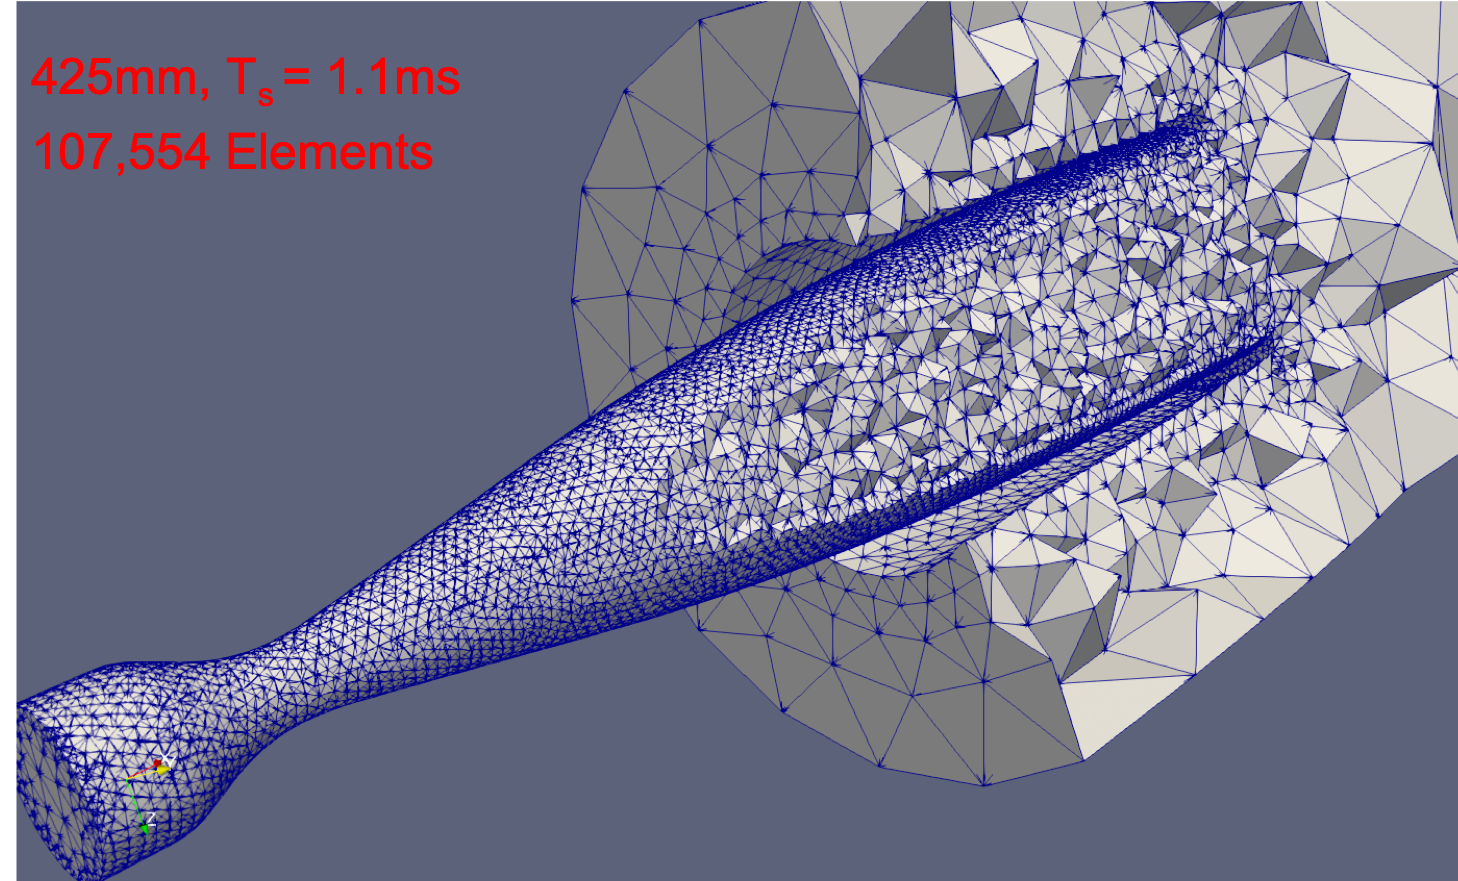
\includegraphics[width=.5\textwidth]{figures/nozzlegrid_annotated2.png}\\
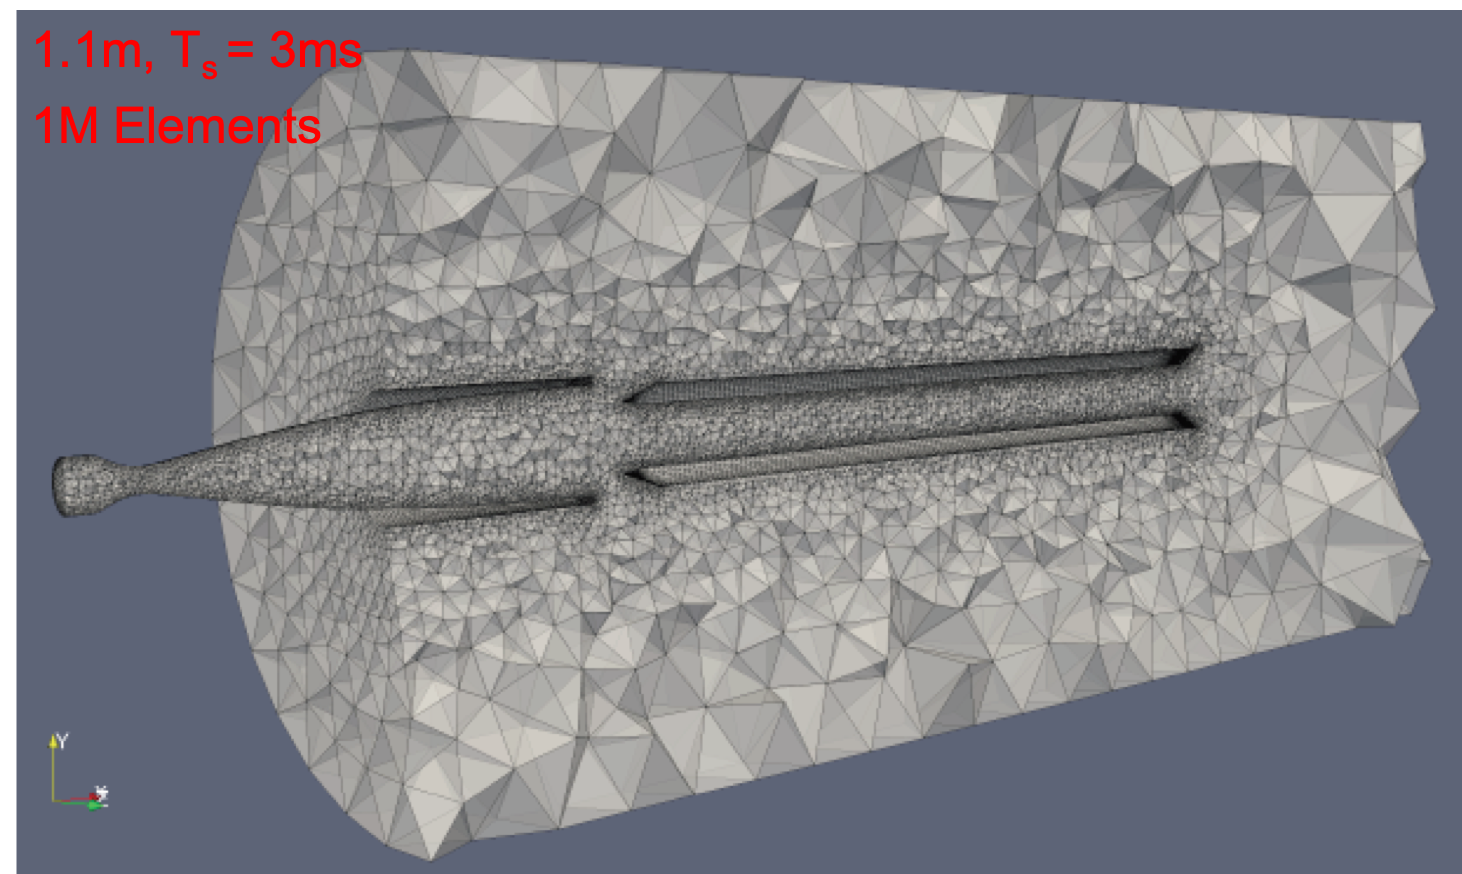
\includegraphics[width=.5\textwidth]{figures/y1grid_annotated.png}\\
\vspace{-10pt}
\begin{center}
 \prj{\tiny}{M.~Smith}
\end{center}
\end{multicols}
\end{frame}

\begin{frame}\frametitle{About grid and element refinement}
\begin{multicols}{2}
\begin{itemize}
\item Determine grid spacing ($h$), and polynomal order ($P$).
\item Refinement is triple whammy:
\begin{itemize}
\item $\Delta{T_s} \approx O(h / P^2)$
\item h-refinement increases $N_e$, $N_s$.
\item P-refinment increases $N_s$, $C_e$
\item Increased MPI message sizes
\end{itemize}
\item Goal: Fix biggest $h$ and lowest $P$ that sufficiently resolve the features and physics.
\end{itemize}
\vspace{15pt}
\end{multicols}
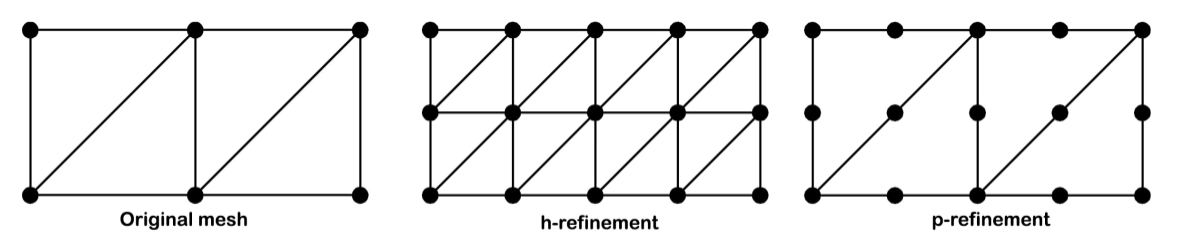
\includegraphics[width=\textwidth]{figures/hpcartoon.png}\\
\begin{center}
\href{https://deust.wordpress.com/2014/11/30/h-method-p-method/}{\textcolor{blue}{\textit{https://deust.wordpress.com/2014/11/30/h-method-p-method/}}}
\end{center}
\end{frame}

\begin{frame}\frametitle{About grid and element refinement}
\begin{multicols}{2}
\begin{itemize}
\item Determine grid spacing ($h$), and polynomal order ($P$).
\item Refinement is triple whammy:
\begin{itemize}
\item $\Delta{T_s} \approx O(h / P^2)$
\item h-refinement increases $N_e$, $N_s$
\item P-refinment increases $N_s$, $C_e$
\item Increased MPI message sizes
\end{itemize}
\item Goal: Fix biggest $h$ and lowest $P$ that sufficiently resolve the features and physics.
\end{itemize}
\end{multicols}
\begin{center}
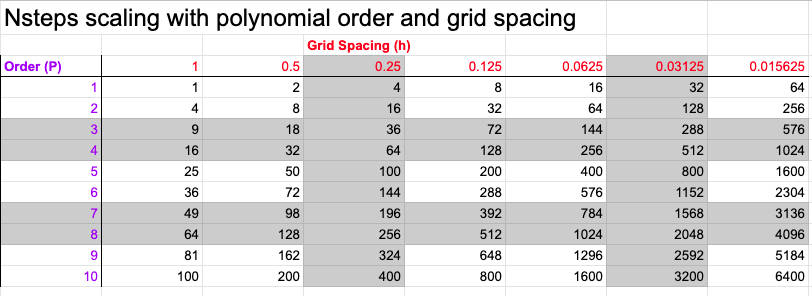
\includegraphics[width=.9\textwidth]{figures/hprefinement_steps.png}
\end{center}
\end{frame}

\begin{frame}\frametitle{About grid and element refinement}
\begin{multicols}{2}
\begin{itemize}
\item Determine grid spacing ($h$), and polynomal order ($P$).
\item Refinement is triple whammy:
\begin{itemize}
\item $\Delta{T_s} \approx O(h / P^2)$
\item h-refinement increases $N_e$, $N_s$.
\end{itemize}
\hspace{-20pt}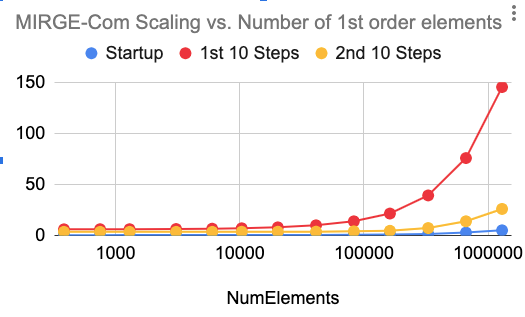
\includegraphics[width=.45\textwidth]{figures/scaling_nelements2.png}
\columnbreak
\begin{itemize}
\item P-refinment increases $N_s$, $C_e$
\item Increased MPI message sizes
\end{itemize}
\item Goal: Fix biggest $h$ and lowest $P$ that sufficiently resolve the features and physics.
\end{itemize}
%\begin{center}
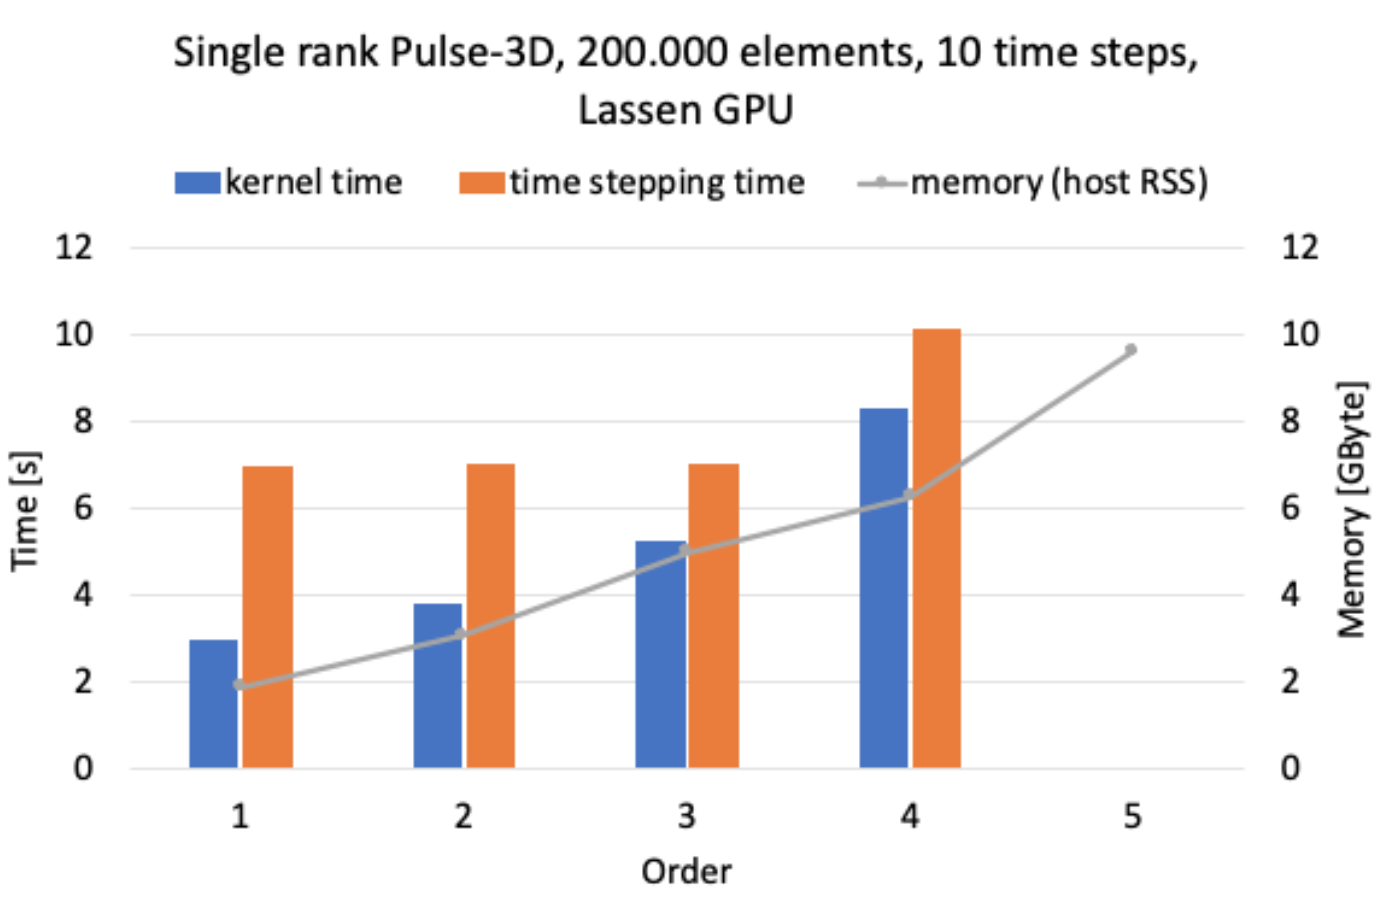
\includegraphics[width=.5\textwidth]{figures/prefinement_impact.png}\\
\begin{center}
\vspace{-15pt}
 \prj{\tiny}{M.~Diener}
\end{center}
\end{multicols}
\end{frame}

\begin{frame}\frametitle{Performance snapshot of production capability}
\begin{multicols}{2}
\begin{itemize}
\item Single component gas
\item Euler + Shock-capturing
\item RK4 timestepping
\item Nozzle-only grid
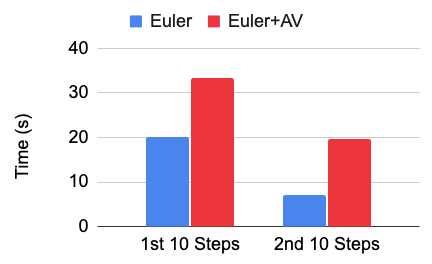
\includegraphics[width=.5\textwidth]{figures/AVCost.png}
\end{itemize}
\columnbreak
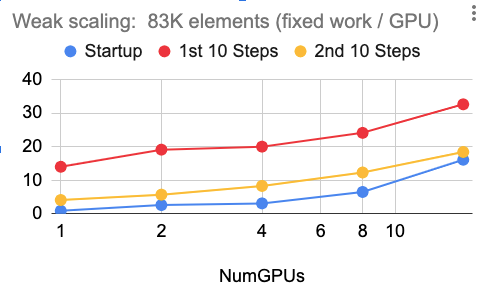
\includegraphics[width=.5\textwidth]{figures/weak_scaling_gpu.png}
\end{multicols}
\begin{center}
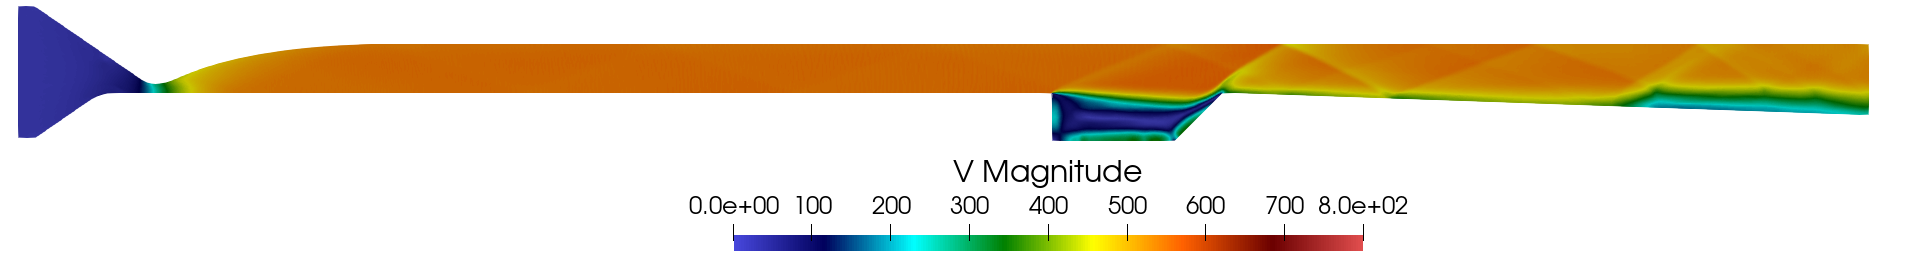
\includegraphics[width=\textwidth]{figures/shock_cap.png}\\
 \prj{\tiny}{Wyatt Hagen}
\end{center}
\end{frame}

\begin{frame}\frametitle{Resource estimation}
\begin{center}
Inviscid flow + shock capturing (1.8s / step)
\end{center}
\begin{multicols}{2}
\begin{itemize}
\item Nozzle-only grid:
\begin{itemize}
\item $\Delta{T_s} = 10^{-8}$
\item $N_s = 1.2\mathtt{ms} / 10^{-8} =  120$K
\item $T_w \approx 2.5$ days on 1GPU
\end{itemize}
\hspace{-20pt}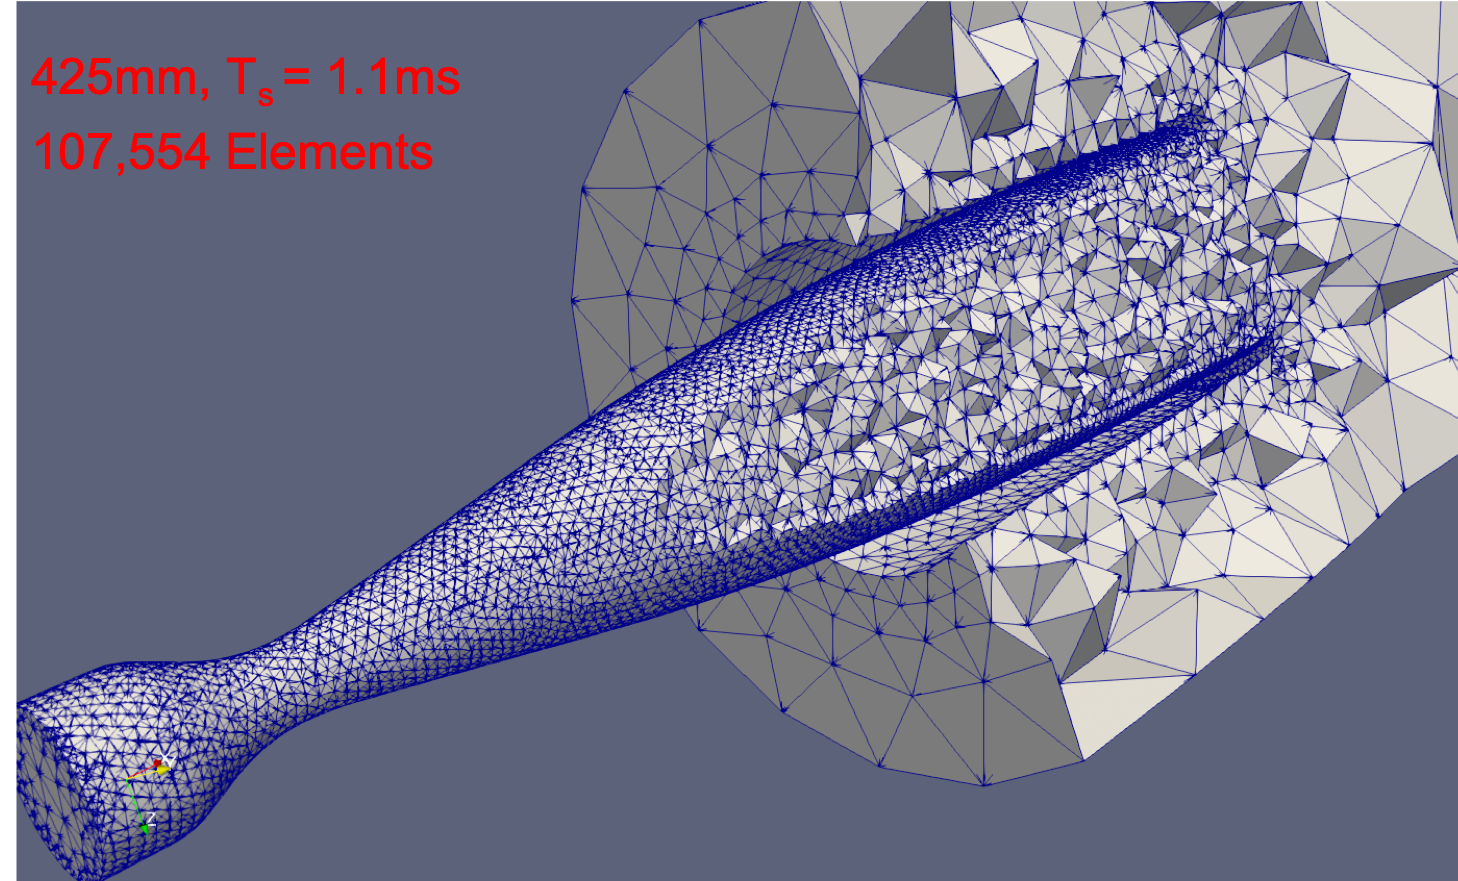
\includegraphics[width=.45\textwidth]{figures/nozzlegrid_annotated2.png}
\columnbreak
\item Full Y1 grid:
\begin{itemize}
\item $\Delta{T_s} \approx 10^{-9}$
\item $N_s = 3\mathtt{ms} / 10^{-9} = 3$M
\item $T_w \approx 60$ days on 10GPUs
\end{itemize}
\end{itemize}
\hspace{5pt}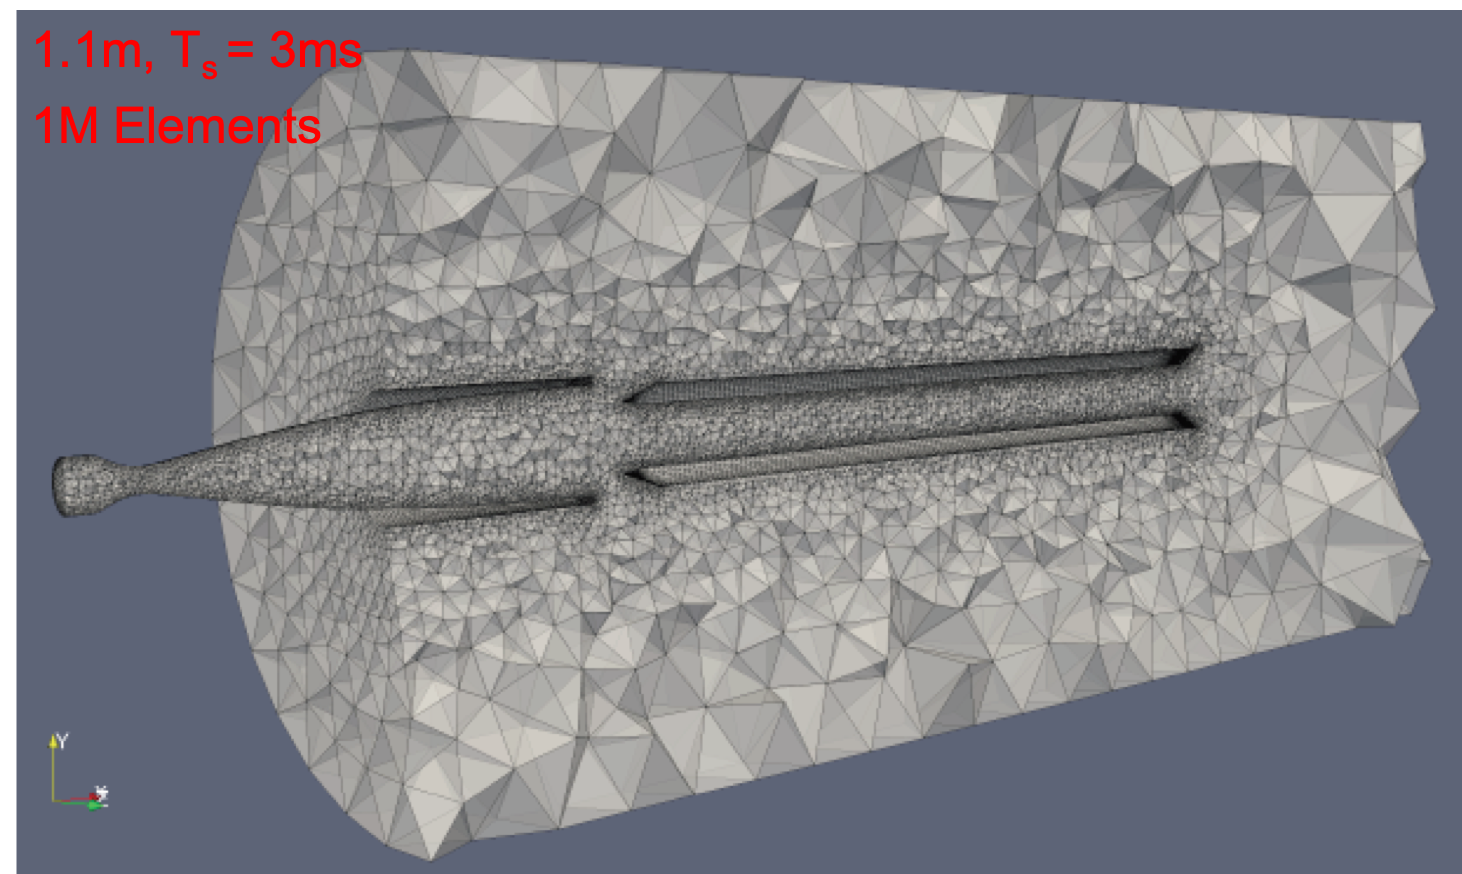
\includegraphics[width=.45\textwidth]{figures/y1grid_annotated.png}
\end{multicols}
\end{frame}

% What computational resource?
% Constraints
% - Developer time (at feature development/eval)
% - Prediction deadline (Sept)
% Observations
%  - talk about the floor

% Resource needs summary and what could go wrong?
% Underestimate DT, h (or Nel), p, cost of NS
% Software latency for MPI communication
% Significant feature adds

% Tracking performance
% Talk up the data summary

% Development TODO:
%  - Viscous fluxes
%  - Viscous wall boundaries
%  - Wall coupling

% Resource estimations/predictions:
%  - Use the smallest resource possible ($$)
%  - Estimate the required resource
%  - Estimate a problem size based on available resource
%  - Adapt to changing resource availability, impact awareness
% Understand the impact of features on resource needs
%  - physics capabilities
%  - number of elements (problem size)
%    - h-refinement
%    - physical domain size
%  - polynomial order (p-refinement)
% Related - scaling
%  - Can I get my answer faster with more resources?
%  - Can I get an answer for a bigger problem in the same amount of time with more resources?
% In time? (September review)
%  - Inviscid flow-through
%  - NS flow-through w/injection
%  - Y1 Simulation
%    - probably requires more in resolution
%    - more elements means more resources
% LASSEN:
% Interconnect: IB EDR (Bi-dir 100Gbps) ~ 10GB/s
% Our message sizes are dinky - 120B/triangle 
% TODO : NAME
% Copy, s/NAME/yourname/
%======================================================================
\begin{frame}\frametitle{In time to matter?}
\begin{itemize}
\item Target: NS flow-through by August (w/ wall model?)
\item What could go wrong:
\begin{itemize}
\item Performance miss: Lazy eval, DAG, transforms \& fusion, MPI
\item Development miss: NS + wall model
\end{itemize}
\item Help is on the way:
\begin{itemize}
\item Concerted effort on performance and monitoring \prj{\tiny}{M. Diener, CEESD}
\item Lazy eval \prj{\tiny}{Kaushik Kulkarni}
\item DAG \prj{\tiny}{Vincent Wells}
\item Tagging \& transforms \prj{\tiny}{Nick Christensen} 
\item MPI performance and modeling \prj{\tiny}{Shelby Lockhart}
\item Absolute kernel performance and scaling \prj{\tiny}{Zane Fink}
\end{itemize}
\end{itemize}
\end{frame}

